\documentclass{article}
\usepackage[utf8]{inputenc}
\usepackage[top=1.25in, bottom=1.25in, left=1.5in, right=1.5in]{geometry}
\usepackage{pgfplots}


\pgfplotsset{
  compat=newest,
  xlabel near ticks,
  ylabel near ticks
}

\begin{document}
\section*{Análise de Utilizadores e Tarefas}

No âmbito do desenvolvimento do projeto, foi necessário identificar e caracterizar os utilizadores alvo, bem como os seus hábitos e necessidades. Assim para este fim, decidimos elaborar um pequeno questionário para responder às onze perguntas comuns que devem ser respondidas aquando da análise do utilizador de uma aplicação. Este relatório visa então expor os resultados do questionário e as respostas às onze perguntas.\\
O questionário era constituído por 25 perguntas e aquando da elaboração deste relatório, foi respondido por 94 pessoas.

\subsection*{Quem vai utilizar o sistema?}
Do que é possível retirar da primeira parte do questionário, o público alvo é constituído maioritariamente por jovens adultos com idades compreendidas entre os 18 e 29 anos (86\% dos inquiridos, como é possível verificar a partir dos resultados à pergunta 2) com o grau de escolaridade referente ao ensino Secundário e Superior (58,24\% e 38,46\% respetivamente, como se verifica nos resultados à pergunta 3). A frequência de idas a bares situasse entre a 1 vez por ano e a 1 vez por semana(verificado as respostas à pergunta 4). Sendo que maioritariamente consome Cerveja/Vinho e Refrigerantes(62,34\% e 54,55\% respetivamente, como é possível verificar na pergunta 5) e a maioria frequenta bares com amigos (97,40\% como se verifica na pergunta 6).
\subsection*{Que tarefas executam atualmente?}
Quando vão a um bar, pergunta número 7, os inquiridos demonstraram uma preferência por socializar (94.37\% dos inquiridos selecionaram esta opção ), beber e comer (69\%) e ouvir música (57.75\%).

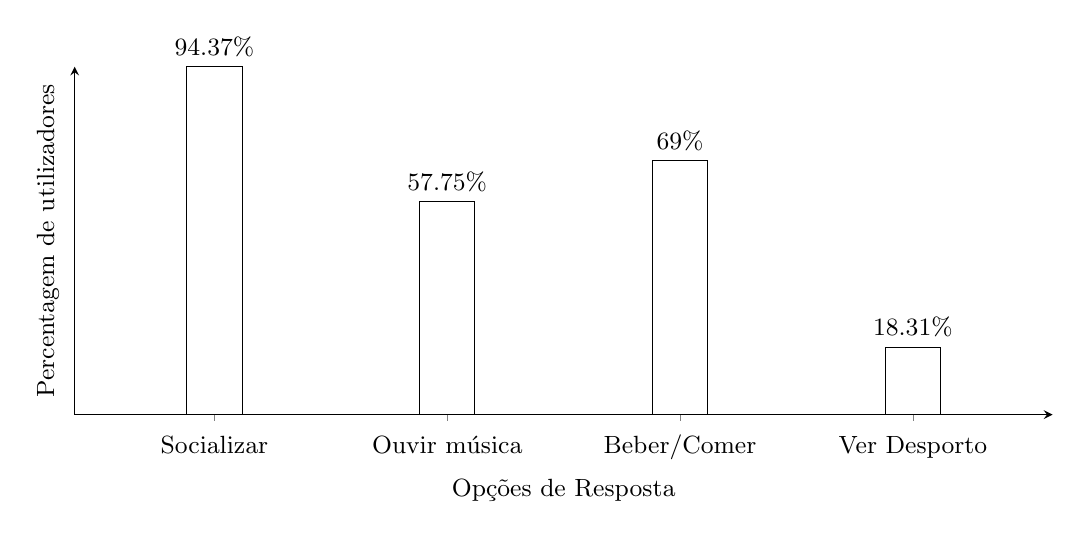
\begin{tikzpicture}[font=\small]
	\begin{axis}[
		ybar,
      	bar width=20pt,
      	width=14cm,
      	height=6cm,
		xlabel={Opções de Resposta},
      	ylabel={Percentagem de utilizadores},
      	ymin=0,
      	ytick=\empty,
      	xtick=data,
      	axis x line=bottom,
      	axis y line=left,
      	enlarge x limits=0.2,
      	symbolic x coords={Socializar, Ouvir música, Beber/Comer, Ver Desporto},
      	xticklabel style={anchor=base,yshift=-\baselineskip},
      	nodes near coords={\pgfmathprintnumber\pgfplotspointmeta\%}
    ]
    \addplot[fill=white] coordinates {
    		(Socializar,94.37)
    		(Ouvir música,57.75)
   		(Beber/Comer,69)
    		(Ver Desporto,18.31)
	};
	\end{axis}
\end{tikzpicture}

\subsection*{Que tarefas são desejáveis?}
Como é possível verificar nas respostas à pergunta 25, os inquiridos mostraram interesse em que a mesa barISTa tivesse funcionalidades como o sistema de votação para música ambiente (70.67\% do inquiridos), a sugestão automática de bebidas consoante os gostos do utilizador (69,33\%), um dispositivo de medição de álcool (65,33\%), uma coletânea de jogos de bebida (58,67\%) e capacidade de pedir um cocktail personalizado(56\%).
\subsection*{Como se aprendem as tarefas?}
Aquando de aprender a utilizar a um sistema eletrónico novo (o que é o caso da mesa barISTa), 92,96\% dos questionados disse que aprendia por experiência de utilização, sendo que uma minoria (29,58\%) pede ajuda a terceiros, como se verifica nas respostas à pergunta 20.
\subsection*{Onde são desempenhadas as tarefas?}
Como seria de esperar, as tarefas desempenham-se num bar. Os inquiridos enquadram o ambiente típico de um bar no centro das escalas de luminosidade e sonoridade (2,94 e 3,26 respetivamente numa escala de 1 a 5, na pergunta 9). Tipicamente fazem pedidos ao balcão (67,4\% dos inquiridos, na pergunta 10).
\subsection*{Qual a relação entre o utilizador e a informação?}
Nas perguntas 23 e 24, respetivamente, concluímos que a maioria(69,33\%) estaria interessada na existência de uma conta com as suas preferências, estando dispostos a partilhar algumas informações pessoais como o seu nome(73,33\%), gostos(66,67\%),e-mail e idade(cerca de 55\%).
\subsection*{Que outros instrumentos tem o utilizador?}
Como é possível verificar na pergunta 11, quando questionados sobre os instrumentos utilizados na escolha do pedido, a maioria respondeu que já possuía ideias pré-definidas em relação ao seu pedido, aquando da ida ao bar. Logo, optam pela não utilização de instrumentos(63.38\%). No entanto, não tendo ideias pré-definidas, recorrem à carta/menu(56.34\%) ou à sugestão de conhecidos(52.11\%).\\

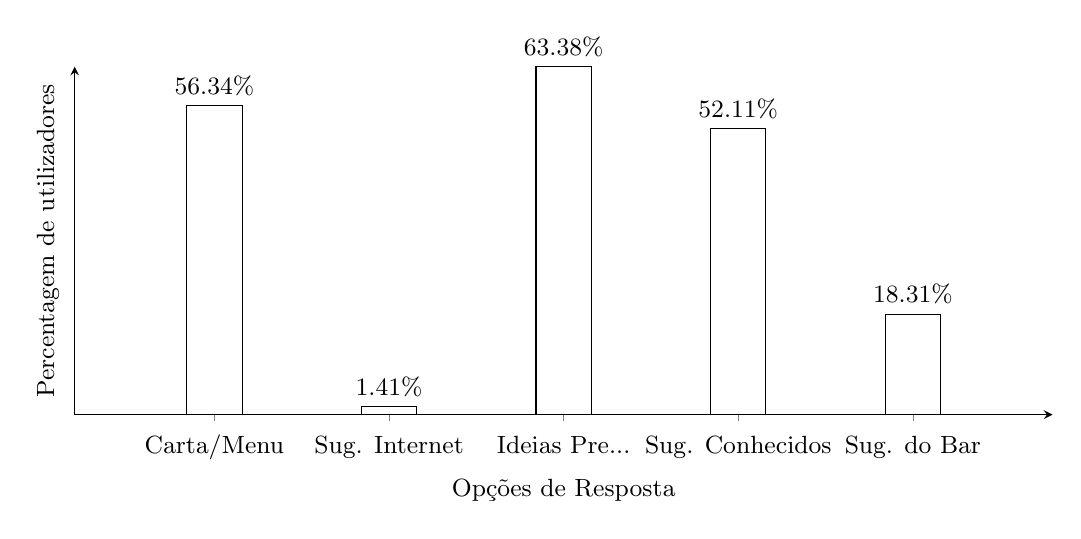
\begin{tikzpicture}[font=\small]
	\begin{axis}[
		ybar,
      	bar width=20pt,
      	width=14cm,
      	height=6cm,
		xlabel={Opções de Resposta},
      	ylabel={Percentagem de utilizadores},
      	ymin=0,
      	ytick=\empty,
      	xtick=data,
      	axis x line=bottom,
      	axis y line=left,
      	enlarge x limits=0.2,
      	symbolic x coords={Carta/Menu, Sug. Internet, Ideias Pre..., Sug. Conhecidos, Sug. do Bar},
      	xticklabel style={anchor=base,yshift=-\baselineskip},
      	nodes near coords={\pgfmathprintnumber\pgfplotspointmeta\%}
    ]
    \addplot[fill=white] coordinates {
    		(Carta/Menu, 56.34)
    		(Sug. Internet,1.41)
   		(Ideias Pre...,63.38)
    		(Sug. Conhecidos,52.11)
    		(Sug. do Bar, 18.31)
	};
	\end{axis}
\end{tikzpicture}

\subsection*{Como comunicam os utilizadores entre si?}
A maioria dos inquiridos, como se pode concluir a partir dos resultados obtidos à pergunta 16, comunica entre si pessoalmente(97,37\%), sendo que uma pequena minoria opta comunicar via eletrónica.
\subsection*{Qual a frequência de desempenho das tarefas?}
Relativamente à utilização de dispositivos eletrónicos, a maioria recorre aos mesmos várias vezes ao dia(71,43\%, como se consegue averiguar pelas respostas à pergunta 19 ).
Num segundo plano, a frequência de idas a bares, pelos questionados, situasse entre 1 vez por ano e 1 vez por semana, sendo que a maioria opta por não conhecer pessoas novas (resultados da pergunta 4 e 15 respetivamente).
\subsection*{Quais as restrições de tempo impostas?}
Os utilizadores têm preferência por um serviço de atendimento rápido(entre 1 a 5 minutos para que o seu pedido seja atendido, confirmado pelas respostas da pergunta 12). Para além disso, privilegiam um serviço operável entre 1 a 3 horas( a maioria dos utilizadores permanece entre 1 a 3 horas num bar, como é possível verificar pelas respostas à pergunta 8).
\subsection*{O que acontece se algo correr mal?}
Deparados com incoerências no seu pedido, grande parte dos inquiridos opta por retornar o pedido e voltar a efetua-lo novamente(90,91\%, resultados à pergunta 18). Como é possível verificar pelas respostas à pergunta 17, quando o seu atendimento se prolonga mais que o normal, os utilizadores preferem avisar os empregados(55,84\%) ou então esperar (36,361\%).

\section*{Funcionalidades a ser implementadas}

Da lista de funcionalidades propostas e mais votadas (apresentadas na resposta à questão "Que tarefas são desejáveis?" das 11 perguntas), selecionamos três que nos pareceram que seriam mais úteis e que tirariam mais proveito das capacidades da mesa interativa.

\subsection*{Cocktail personalizado}
Esta funcionalidade permite ao utilizador criar o um cocktail ao seu gosto, dizendo os ingredientes de uma lista pré definida.\\

\subsection*{Votação para Música Ambiente}
A votação para musica ambiente é um funcionalidade que permite ao utilizadores do o bar escolherem democraticamente que música de fundo passa. Isso permite melhorar a experiência do utilizador pois podem ouvir a música que lhes agrade.\\

\subsection*{Coletânea de jogos de bebida}
Uma coletânea de jogos de bebida disponíveis na mesa interativa permite aos utilizadores terem mais opções de diversão quando vão a um bar para além da tradicional socialização.\\



\end{document}